\documentclass[12pt]{tcc}
\usepackage[brazil]{babel}
\usepackage[T1]{fontenc}
%\usepackage[brazilian,hyperpageref]{backref}
\usepackage[hidelinks]{hyperref}
\usepackage[pt-BR]{datetime2}
\DTMlangsetup{showdayofmonth=false}
\usepackage[portuguese,ruled,linesnumbered,algochapter,titlenumbered]{algorithm2e}
\usepackage{listings}
\usepackage{xcolor}
\usepackage[toc,page]{appendix}
\definecolor{mygreen}{RGB}{64,100,64}

% Define TypeScript language style
\lstdefinelanguage{TypeScript}{
    keywords=[1]{import, from, export, static, public, implements, extends, class, extends, private, void, constructor, super, this, async, await, for, of, let, in, return, console, log, abstract},
    keywordstyle=[1]\color{blue},
    keywords=[3]{MockTime, Promise, IPersister, Task, CompositeTask, BasicPersister, Resource, Project, MockTask, Metric, DeltaTimeMetric, ProcessMemoryMetric, Set, JSON, Math, any, string},
    keywordstyle=[3]\color{mygreen},
    ndkeywords={true, false, catch, function, null, undefined},
    ndkeywordstyle=\color{darkgray},
    identifierstyle=\color{black},
    sensitive=true,
    comment=[l]{//},
    morecomment=[s]{/*}{*/},
    commentstyle=\color{green}\ttfamily,
    stringstyle=\color{red}\ttfamily,
    morestring=[b]',
    morestring=[b]",
	lineskip=-1pt
}

\lstset{
    backgroundcolor=\color[gray]{0.9},
    numbers=left,
    stepnumber=1,
    numberstyle=\small\ttfamily\color{gray},
    numbersep=5pt,
    aboveskip=10pt,
    belowskip=10pt
}

% As figuras ficam armazenadas na pasta figuras.
\graphicspath{{./figures/}}

% Informações do trabalho
\newcommand\dtitle{Framework para Análise de Desempenho de Consultas Web}
\newcommand\dauthor{Filipe Shanom Glathardt de Azeredo Xavier\\Matheus dos Santos Moura\\Radhanama Dasa de Maria Moraes Mesiano}
\newcommand\dadvisor{Renato Campos Mauro}

% Definição de acronimos
\newacro{TCC}{Trabalho de Conclusão de Curso}
\newacro{QoS}{qualidade de serviço}
\newacro{API}{\emph{Application Programming Interface}}

\begin{document}
\pagenumbering{gobble}
\pagenumbering{roman}

\dcover

\dcoverback
	
\dlibrary{ficha.pdf}
		
\ddedicatory{
	\raggedleft \normalsize Dedico este trabalho aos futuros pesquisadores, cuja as descobertas e avanços sejam impulsionados por esse trabalho. Que esse framework sirva de apoio para que possam avaliar o desempenho de suas próximas pesquisas, e que isso gere impactos positivos na sociedade.
	Dedicamos também aos nossos professores, cuja orientação nos trouxe os conhecimentos necessários para realização desse projeto. Seus ensinamentos foram fundamentais para nos capacitar a desenvolver esse trabalho.
}

\dacknowledgment{
	Agradece-se à CAPES, CNPq e FAPERJ pelo financiamento parcial desta pesquisa.\\
	\\
	Agradece-se também à plataforma Scopus e à CAPES pelas valiosas fontes de pesquisa que foram extremamente importantes para a fundação teórica deste trabalho. 
	Também desejo expressar minha gratidão aos meus colegas de grupo, cuja colaboração e esforço conjunto foram fundamentais em todas as etapas do projeto. A colaboração de cada um de vocês foi de extrema importância.
	Por fim, não podemos deixar de agradecer aos nossos familiares, cujo apoio, encorajamento e compreensão nos motivaram a superar os desafios propostos.
}

\dresumo{
Desde a popularização dos smartphones a quantidade de dados gerados cresce sem precedentes, de modo que até torna a definição de grande volume de dados difícil, devido a sua rápida obsolescência.
Dentro deste contexto, aplicações Web cliente-servidor as quais ofertam visualização de dados para grandes volumes sofrem muitas vezes com limitações de recursos computacionais no lado do cliente.
Além disso, seus desenvolvedores encontram desafios ao avaliar o consumo dos recursos, pois, há grandes dificuldades em cobrir a ampla gama de configurações que existem no lado do cliente.
Por outro lado, também existe uma carência por ferramentas as quais permitam esse tipo de avaliação, e que possuam funcionalidades para auxiliar a coleta de métricas de execuções da aplicação realizadas por voluntários.
A fim de solucionar estes problemas, propomos um framework para o ecossistema JavaScript capaz de executar provas de conceito, enquanto realiza a coleta de métricas de desempenho e consumo de recursos computacionais, o qual também seja facilmente extensível para necessidades específicas do projeto e que auxilie no processo de avaliação realizado por voluntários.
}{big data; Web; visualização de dados; avaliação de desempenho; consumo de recursos; framework}

\dabstract{
Since the popularization of smartphones, the amount of data generated has grown unprecedentedly, so that it even makes it difficult to define how big big data is, due to its rapid obsolescence.
In this context, client-server Web applications which offer data visualization for big data often suffer from limitations of computational resources on the client side.
In addition, its developers find challenges when evaluating resource consumption, as there are great difficulties in covering a wide range of configurations on the client side.
On the other hand, there is also a lack of tools that guarantee this type of evaluation, and contain features to help collect application execution metrics performed by volunteers.
In order to solve these problems, we propose a framework for the JavaScript ecosystem capable of executing proofs of concept, while collecting performance indicators and consumption of computational resources, which is also easily extensible for specific needs of the project and that helps the estimation process carried out by volunteers.
}{big data; Web; data visualization; performance evaluation; resource consumption; framework}

\dtables
	

\pagenumbering{arabic}
\justifying
	
\chapter{Introdução}
\label{cap:intro}

Desde o começo da era da informação e principalmente após a popularização dos smartphones a quantidade de informações geradas cresce em um ritmo sem precedentes \citep{Gandomi2015Beyond}.
Este cenário com disponibilidade de grandes volumes de dados (do inglês, \emph{big data}), criou diversas oportunidades para modelos de negócios voltados para o uso desses dados.
Empresas como Google e Meta (antigo Facebook), se tornaram gigantes do mercado explorando estes modelos de negócios baseados em dados.

Entretanto, o manuseio de grandes volumes de dados necessita de cuidados especiais.
Pois, eles podem superar o tamanho de qualquer memória principal ou secundária as quais são encontradas no mercado.
Alguns exemplos desses tratamentos especiais para o manuseio de grandes volumes de dados são o modelo de programação MapReduce \citep{Dean2008MapReduce} e o sistema de armazenamento de objetos Haystack \citep{Beaver2010Finding}.
Portanto, os sistemas que manuseiam grandes volumes de dados precisam ser planejados para sua carga de trabalho.

Por outro lado, aplicações Web com arquitetura cliente-servidor sofrem com o problema da ampla variedade de configurações tanto de hardware quanto de software no lado do cliente.
E, os desenvolvedores, por sua vez, não possuem diversos tipos de ambientes para exercitar suas aplicações, o que pode levar a problemas com alguns tipos de configurações.
Além disso, mesmo quando existe acesso a diferentes tipos de ambiente, é improvável que a equipe de desenvolvimento tenha acesso direto, sendo necessário a colaboração de alguém externo.

A fim de atenuar estes problemas, estamos propondo um framework o qual um desenvolvedor de uma aplicação Web cliente-servidor seja capaz de facilmente obter métricas e estatísticas sobre provas de conceito, as quais, precisam ser executadas em diversas configurações de clientes por voluntários.
Por exemplo, considere uma aplicação Web a qual precisa trafegar um volume suficientemente grande de dados entre o cliente e o servidor, de modo que, seja impossível de manter todos dados em cache no lado do cliente.

Para realizar o tráfego de dados, uma equipe de desenvolvimento considera as seguintes opções de formato de arquivo: CSV, JSON, Arrow e Parquet.
Com o objetivo de tomar essa decisão, a equipe decide realizar uma análise de desempenho e consumo de recursos em cada uma das abordagens variando os tipos de clientes.
E, para incluir nas avaliações a maior variedade possível de clientes, eles também decidem automatizá-la, de modo que seja possível contar com o auxílio de voluntários.
Porém, com o intuito de tornar isso possível, além da prova de conceito, a equipe ainda precisaria desenvolver como expor, executar e coletar as métricas durante a avaliação. Este é o tipo de cenário para qual o framework está sendo proposto. 

A contribuição principal do ELC é oferecer uma forma fácil e eficaz de realizar a execução de tarefas customizáveis no lado do cliente, e também o registro dos resultados dessas execuções em uma base de dados, também customizável. Dessa forma, seria possível de forma simples resolver o problema da equipe de desenvolvimento.

Ademais, o framework por padrão possui algumas métricas básicas implementadas, como tempo gasto na tarefa, memória utilizada e a identificação do ambiente de execução, e os dados são armazenados em uma planilha online para fácil obtenção e análise.

Deste modo, o desenvolvedor pode focar nas provas de conceito e na obtenção de ambientes e voluntários, ao invés do desenvolvimento de infraestrutura para realização das avaliações.


O trabalho está dividido em cinco capítulos.
O capítulo \ref{cap:met_pesquisa} e \ref{sec:trab_relacionados} correspondem a metodologia da pesquisa e trabalhos relacionados encontrados no campo de estudo.
O capítulo \ref{cap:proposta} apresenta a proposta de desenvolvimento da ferramenta.
Por fim, os capítulos \ref{cap:prova_de_conceito} e \ref{cap:estado_atual} apresenta o estado atual do framework e o cronograma para a próxima etapa.


\chapter{Fundamentação teórica}
\label{cap:fundamentacao_teorica}
Aqui vai um texto introduzindo a fundamentação teórica

	\section{Evolução da web e a necessidade de performance}
	\label{cap:evolucao-web}
	Inserir texto aqui

	\section{Medição client-side}
	\label{cap:medicao-client-side}
	Inserir texto aqui

	\section{JS nos navegadores}
	\label{cap:js}
	Inserir texto aqui

	\section{SOLID - Principio do Open/closed}
	\label{cap:solid}
	Inserir texto aqui

	\section{Padrão de software Composite}
	\label{cap:composite}
	Inserir texto aqui



\chapter{Trabalhos Relacionados}
\label{sec:trabalhos_relacionados}
	\label{sec:trab_relacionados}

	% \item \textbf{Paper 1}: Summary of the first paper goes here. This paragraph provides a concise overview of the paper's objectives, methodology, and key findings.

	\section{Metodologia de Pesquisa}
	\label{cap:met_pesquisa}

	Para a revisão bibliográfica as duas principais ferramentas utilizadas foram: Elicit, um assistente de pesquisa baseado em modelos de transformador pré-treinado generativo (do inglês, \emph{generative pre-trained transformer}) de aprendizado de máquina, e a ferramenta Connected Papers, a qual  gera um grafo de artigos relacionados baseado em cocitações e acoplamento bibliográfico.
	A ferramenta Elicit funciona recebendo uma pergunta em linguagem natural e retornando os trabalhos que considera mais relevantes, junto a um resumo, em uma tabela paginada.
	Deste modo, na tabela \ref{tab:strings-elicit} elencamos todas strings de busca utilizadas no Elicit, e para cada uma delas consultamos até a segunda página da tabela, totalizando 14 trabalhos retornados por string de busca.

	\begin{table}[h!]
	\centering
	\caption{Strings utilizadas na ferramenta Elicit.\label{long}}

	\begin{tabular}{||c||} 
		
	\hline
		Strings de Busca \\
	\hline\hline
	``browsing memory'' \\
	``client side memory performance'' \\
	``client side memory profiling'' \\
	``memory network management web client'' \\
	``memory network performance web client'' \\
	``memory network profiling web client'' \\
	``memory network waste web client'' \\
	``measuring performance in client side'' \\
	``measuring in client side'' \\
	``performance measurement'' \\
	``tools to measure performance in client side'' \\
	``evaluating latency on client side'' \\
	``optimizing web browsing'' \\
	``performance tool web client side'' \\
	``waste resources client side'' \\
	``waste resources web client'' \\
	``web client side memory performance'' \\
	``What are the impacts of memory management in mobile Web Browsing?'' \\
	``What is the state-of-the-art for measuring performance of client side?'' \\
	``What is the state-of-the-art for measuring QoE and memory of Web Browsing?'' \\

	\hline
	\end{tabular}
	\label{tab:strings-elicit}
	\end{table}

	Além disso, três trabalhos encontrados por meio do Elicit foram utilizados como entrada para a ferramenta Connected Papers.
	O Connected Papers é um outro assistente de pesquisa, o qual recebe como entrada o título ou o DOI de um trabalho para gerar um grafo de trabalhos relacionados destacando suas principais conexões e trabalhos influentes.
	As strings de busca utilizadas no Connected Papers estão listadas na tabela \ref{tab:strings-connected-papers}, de modo que, para cada uma, a ferramenta gerou um grafo com 40 trabalhos relacionados, os quais também podem ser visualizados em uma tabela. \\

	\begin{table}[h!]
	\centering

	\caption{Strings utilizadas na ferramenta Connected Papers.}
	\begin{tabular}{||c||} 

	\hline
		Strings de Busca \\
	\hline\hline
	``Measuring Web Latency and Rendering Performance: Method, Tools, and Longitudinal Dataset''\\
	``MemInsight: platform-independent memory debugging for JavaScript''\\
	``Obtaining in-context measurements of cellular network performance''\\
	\hline
	\end{tabular}
	\label{tab:strings-connected-papers}
	\end{table}

	Os critérios usados para filtrar os trabalhos encontrados por meio de ambas as ferramentas estão descritos na figura \ref{fig:fluxo-leitura}.
	Em suma, após a leitura do resumo de cada trabalho, três critérios são avaliados, sendo cada um deles um filtro.
	O qual indica se o trabalho não tem relação suficiente com o tema, se é necessário ler a introdução para a tomada da decisão ou se é um trabalho o qual a leitura completa deve ser realizada.

	\begin{figure}[!ht]
		\centering
		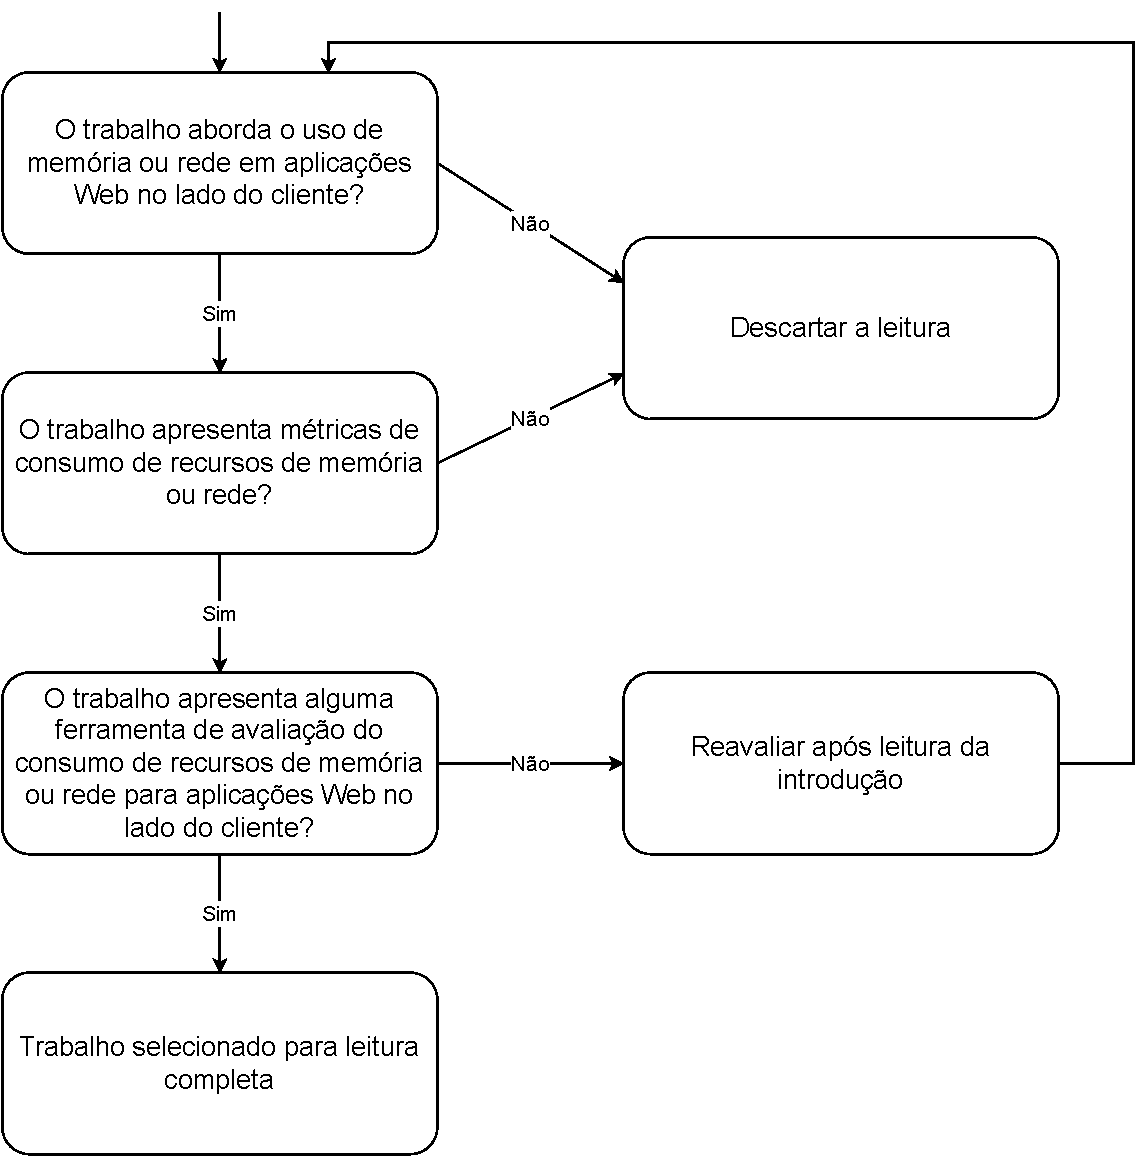
\includegraphics[width=0.6\textwidth]{figures/fluxo-decisao-leitura.pdf}
		\caption{Critérios utilizados para seleção de trabalhos para leitura.}
		\label{fig:fluxo-leitura}
	\end{figure}


	\begin{table}[!ht]
		\centering
		\caption{Total de trabalhos encontrados}
		\begin{tabular}{l  c L{1.5cm} R{1.5cm}}
			\toprule
			\textbf{Ferramenta} & \textbf{Trabalhos Encontrados} \\
			\midrule
			Elicit  &  280  \\
			Connected Papers  &  120  \\
			\midrule
			Total  &  400  \\
			\bottomrule
		\end{tabular}
		\label{tab:trabalhos-encontrados}
	\end{table}


	\section{Ferramentas Para Medição no Lado do Cliente}
	Utilizando os métodos descritos na seção anterior do trabalho, conseguimos levantar um panorama geral dos frameworks e soluções existentes e propostos à academia, assim como classificá-los utilizando alguns parâmetros, afim de entender se a nossa proposta se demonstra complementar ao estado da arte. 
	Os critérios da classificação são: 


	\begin{table}[!ht]
		\centering
		\caption{Critérios de classificação das ferramentas}
		\begin{tabular}{l c L{1.5cm} R{1.5cm}}
			\toprule
			\textbf{Critério} & \textbf{Descrição}\\
			\midrule 
			Arquitetura Simples & Se a arquitetura da ferramenta é de fácil entendimento.\\
			Flexibilidade&Se a ferramenta se adapta em diversos contextos de medição.\\
			Curva de Aprendizado&Se a ferramenta possui uma curva de aprendizado rápida.\\
			Multiplataforma&Se a ferramenta suporta o uso em diversas plataformas.\\
			Persistência&Se a ferramenta persiste dados para análise futura.\\
			\bottomrule
		\end{tabular}
		\label{tab:string-busca-connected-papers}
	\end{table}


	\par Dessa forma, a classificação dos trabalhos selecionados se encontra na tabela abaixo:

		\begin{table}[ht]
			\scriptsize
			\caption{Classificação das ferramentas encontradas} % title of Table
			\centering % used for centering table
			\begin{tabular}{l c c c c c} % centered columns (4 columns)
			\toprule
			\textbf{Plataforma} & \textbf{Arquitetura Simples} & \textbf{Flexibilidade} & \textbf{Curva de Aprendizado} & \textbf{Multiplataforma} & \textbf{Persistência} \\[0.5ex]

			%heading
			\midrule % inserts single horizontal line
			MemInsight & sim & não & sim & sim & não \\
			WePR & não & não & não & sim & sim \\
			Gember & sim & não & sim & não & sim \\
			Mobilyzer & sim & não & não & não & sim \\
			\hline %inserts single line
			\end{tabular}
			\label{table:ferramentas-encontradas} % is used to refer this table in the text
		\end{table}
	

		\subsection{MemInsight}
		\par No contexto de medição de memória, temos a MemInsight \citep{Jensen2015MemInsight}. Essa ferramenta roda de forma independente sobre uma engine Javascript, não sendo necessário um browser para executar, e faz a análise do consumo de memória por meio de um conjunto de medições que visam remontar o ciclo de vida dos objetos em memória, e que permitem a análise de desperdício de recursos durante a execução do programa. 
		\par Analisando a ferramenta, foi observado que ela só trabalha com medição de métricas de memória, não permitindo generalizar consultas de outros tipos, por isso classificamos como não flexível com relação às métricas. Além disso, por ser uma ferramenta com foco em depurar aplicações, não realiza nativamente a persistência e organização desses dados.
		

		\subsection{WePR}
		\par \citep{Asrese2019MeasuringWL} também propôs uma ferramenta para medição no lado do cliente, porém agora com o enfoque em medir métricas de \acr{QoS}, nomeada WePR. No trabalho, ele apresenta um panorama da evolução da web, especialmente de como a latência se desenvolveu nos sites, e sustenta a necessidade desse tipo de medição como forma de melhorar a experiência do usuário, que indicam ser um fator determinante no abandono ou sucesso de um website. A ferramenta foi testada utilizando grandes sites como Google, Youtube e Facebook. 
		\par A arquitetura da ferramenta é distribuída, e consiste basicamente de um coletor, um servidor que fornece os elementos das páginas para medição, múltiplos servidores de renderização gerenciados por um balanceador de carga (do inglês, \emph{load balancer}), e um servidor que cuida da persistência dos dados. Dessa forma, o coletor inicialmente pede ao servidor as URLs dos elementos a serem medidos, e após obter essa resposta, faz o download desses elementos e captura métricas. Posteriormente, envia esses dados medidos e os elementos baixados para o balanceador de carga, e por fim algum dos servidores de renderização envia os dados para persistência.
		\par O enfoque da ferramenta é a análise de desempenho de sites, dessa forma sua arquitetura e usabilidade não foram construídas de forma simples de estender, tornando difícil a utilização da ferramenta em outros contextos. Além disso, não temos a possibilidade de incluir métricas customizadas, o que torna sua análise pouco flexível.
		
		\subsection{Gember}
		\par \citep{Gember2012Obtaining} também traz um estudo sobre medição no lado do cliente, porém dessa vez em clientes móveis, utilizando dados de um provedor de internet e também de experimentos controlados. Esse tipo de medição é muito útil para provedores de internet e desenvolvedores, que precisam entender como suas aplicações se saem interagindo com redes móveis de internet.
		\par Foi desenvolvido no trabalho um protótipo para Android de um medidor de performance para analisar somente quando o dispositivo está ativo, e que é integrado ao app como uma biblioteca. A arquitetura consiste basicamente de um controlador central (servidor), e múltiplos clientes (aparelhos) com o código rodando em seus celulares. Dessa forma, o pesquisador faz uma requisição para esse controlador, e ele coordena a coleta do que foi solicitado nos aparelhos, salvando os resultados no servidor.
		\par O serviço inicialmente coleta latência, taxa de transferência (do inglês, {throughput}) e o tempo de carregamento de páginas Web, é extensível para outras métricas de rede, porém limitado a elas. Outra limitação aqui é a utilização no cliente, que se encontra somente no sistema operacional Android, tornando pouco flexível a utilização dessa ferramenta nos contextos de pesquisas multiplataforma.

		\subsection{Mobilyzer}
		\par Ainda no contexto de medição de rede, se encontra o Mobilyzer \citep{Nikravesh2015Mobilyzer}, uma plataforma aberta para medição de rede em dispositivos móveis. Essa plataforma foi criada com o objetivo de prover uma solução escalável, eficiente e controlável, que fosse possível de ser incorporada tanto a apps em desenvolvimento, quanto em apps que já estão desenvolvidos, para suportar pesquisas e testes em medição de rede. 
		\par Ela funciona utilizando alguns componentes básicos, sendo eles: 
		\begin{enumerate}
			\item Uma biblioteca Android, que é integrada aos aplicativos para coletar as informações e enviar ao servidor. Ela é incorporada direto no código fonte.
			\item Um componente chamado gerenciador de memória, no qual o pesquisador pode inserir medições de forma customizada e mais eficiente. Ele também realiza o agendamento das medições, e também coordena e monitora os dispositivos para que não tenha sobrecarga em nenhum aparelho ou rede medida. 
			\item Um servidor na nuvem, que fica responsável por coletar, analisar aplicando regras e publicar os dados coletados dos dispositivos. Essa arquitetura centralizada simplifica o compartilhamento de dados entre essas etapas, podendo integrar outras ferramentas de análise de dados com a base das coletas.

		\end{enumerate}
		\par Uma dificuldade no uso do Mobilyzer em pesquisas é que essa plataforma também se restringe a plataforma Android. Diminuindo bastante as possibilidades de medição em pesquisas multiplataforma. Além disso, não possui muita flexibilidade com relação às métricas, sendo em sua maior parte métricas de rede.

		\subsection{Nossa Ferramenta}
		\par Após o descrito, podemos posicionar a nossa ferramenta com relação aos critérios que estabelecemos no começo desta seção. Temos um modelo de arquitetura simples que será explicado nas seções futuras deste trabalho, a possibilidade de expandir e construir métricas diversas, uma curva de aprendizado suave, a compatibilidade com múltiplas plataformas pois a coleta das métricas ocorre no navegador, e também a persistência desses dados para futura análise.
		\par Assim, a tabela teria a seguinte configuração após a adição da nossa ferramenta:

		\begin{table}[ht]
			\scriptsize
			\caption{Classificação das ferramentas encontradas com a nossa ferramenta} % title of Table
			\centering % used for centering table
			\begin{tabular}{c c c c c c} % centered columns (4 columns)
			\toprule %inserts double horizontal lines
			\textbf{Plataforma} & \textbf{Arquitetura Simples} & \textbf{Flexibilidade} & \textbf{Curva de Aprendizado} & \textbf{Multiplataforma} & \textbf{Persistência} \\[0.5ex]

			%heading
			\midrule % inserts single horizontal line
			MemInsight & sim & não & sim & sim & não \\
			WePR & não & não & não & sim & sim \\
			Gember & sim & não & sim & não & sim \\
			Mobilyzer & sim & não & não & não & sim \\
			Nossa Ferramenta & sim & sim & sim & sim & sim \\
			\bottomrule %inserts single line
			\end{tabular}
			\label{table:ferramentas-encontradas-com-nossa-ferramenta} % is used to refer this table in the text
		\end{table}

\chapter{Implementação}
\label{cap:implementação}

	O objetivo principal do framework é oferecer uma forma fácil e eficaz de realizar a execução de tarefas no lado do cliente, e o registro dos resultados dessas execuções em uma base de dados.
	Dessa forma, o usuário do framework é capaz de realizar seus experimentos com a colaboração de voluntários mais facilmente, tendo a estrutura básica do projeto. Nessa secção, explicaremos os principais pilares que sustentam a nossa solução, definindo os elementos que a compõem.

\section{Estudos de caso}

\subsection{Projeto dos números primos}

Projeto no qual utilizamos o el-chupacabra de forma mais completa, inclusive usando o Composite nas tasks.


\subsection{Site dos números primos utilizando o EasyELC}

Exemplo mais simples, customizando o menos possível, e com um uso mais simplificado. Utilizar a estrutura do EasyELC aplicada no site dos números primos.

\section{Diagrama de Casos de Uso}
\label{cap:diagrama_de_caso_de_uso}

O diagrama de casos de uso é o diagrama responsável por prever como a ferramenta será utilizada, embasando futuramente o desenvolvimento e os testes da aplicação. No caso do ELC, temos os atores ...

\begin{figure}[!ht]
	\centering
	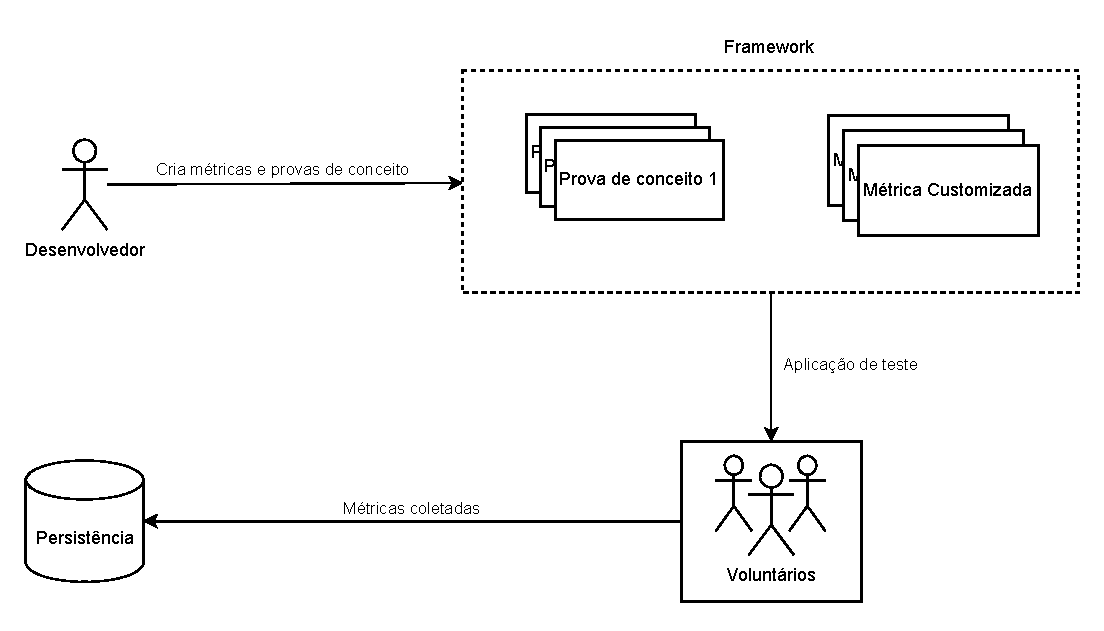
\includegraphics[width=0.6\textwidth]{figures/diagrama-informal.pdf}
	\caption{Principal fluxo de uso, onde um desenvolver avalia um conjunto de provas de conceitos com o auxílio de voluntários externos ao desenvolvimento.}
	\label{fig:diagrama-informal}
\end{figure}

	
\section{Diagrama de Classes}
\label{cap:diagrama_de_classe}


O diagrama conceitual detalhado define a arquitetura e estrutura dos módulos do framework.
Nele há a definição dos principais aspectos práticos para a implementação, por exemplo, são definidas as árvores de herança e principais métodos que precisam ser implementados por usuários.
Além disso, ele também define a camada de persistência para resolver o problema da coleta de métricas de execuções realizadas por voluntários de forma remota.
Abaixo, está uma descrição de cada elemento do diagrama.

\begin{figure}[!ht]
	\centering
	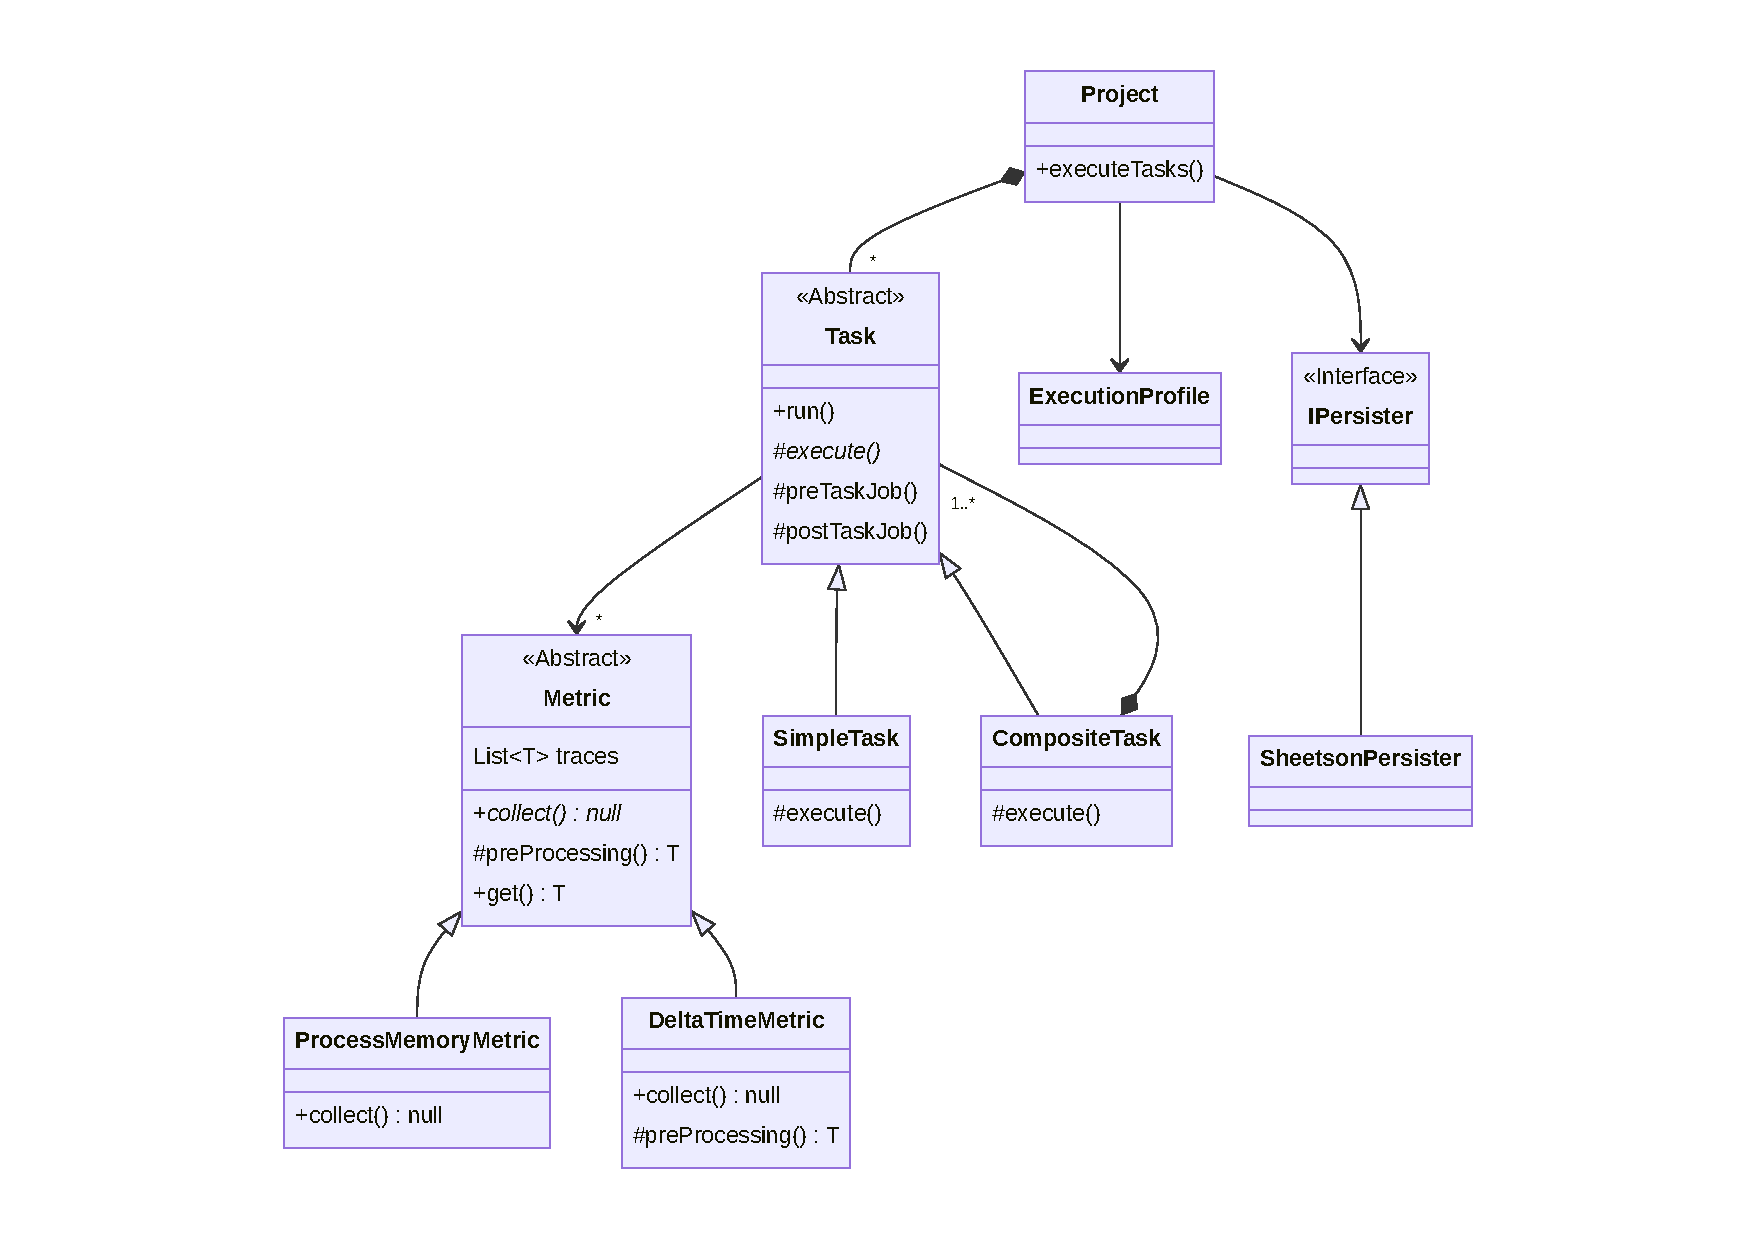
\includegraphics[width=0.9\textwidth]{figures/diagrama-classes.pdf}
	\caption{Diagrama conceitual detalhado do framework.}
	\label{fig:diag-classes}
\end{figure}


\begin{description}
	\item[Project:] Responsável por coordenar a execução das análises e encaminhar suas métricas para a camada de persistência.
	\item[ExecutionProfile:] Responsável pela coleta de dados sobre o ambiente de execução.
	\item[Task:] Responsável por definir a rotina de execução das tarefas e seus métodos públicos.
	\item[SimpleTask:] Classe base para implementação de uma tarefa.
	\item[CompositeTask:] Classe base para implementação de tarefas compostas.
	\item[Metric:] Responsável por definir a rotina para coleta de uma métrica e seus métodos públicos.
	\item[ProcessMemoryMetric:] Implementação de uma métrica para medir o consumo de memória.
	\item[DeltaTimeMetric:] Implementação de uma métrica para medir tempo gasto em uma tarefa.
	\item[IPersister:] Responsável por definir a interface pública da camada de persistência.
	\item[SheetsonPersister:] Implementação da camada de persistência a qual utiliza o Google Sheets\footnote{https://www.google.com/sheets/about}.
\end{description}

\section{Arquitetura}
\label{cap:diagrama_de_arq}

A ferramenta foi implementada utilizando uma arquitetura modular, e seguindo fortemente o conceito do aberto/fechado (open/closed), trazido pelo SOLID (citar fundamentação teórica). Dessa forma, todas as relações entre as classes e módulos se dão através de interfaces, abstraindo o funcionamento interno de cada elemento. Isso contribui significativamente para a manutenabilidade do código, pois diminui as chances de problemas de compatibilidade entre as implementações caso alguma premissa seja alterada.

Inicialmente, a ferramenta se estrutura em seis módulos principais: o Módulo de Projeto (Project), Módulo de Perfil de Execução (ExecutionProfile), o módulo de Métricas (Metrics), o módulo de Persistência (Persister), o módulo de Tarefas (Tasks) e o Módulo Simplificado (EasyELC). Cada um deles possui sua responsabilidade, como serão descritas nas próximas secções. (atualizar diagrama pra inserir o módulo EasyELC)

\begin{figure}[!ht]
	\centering
	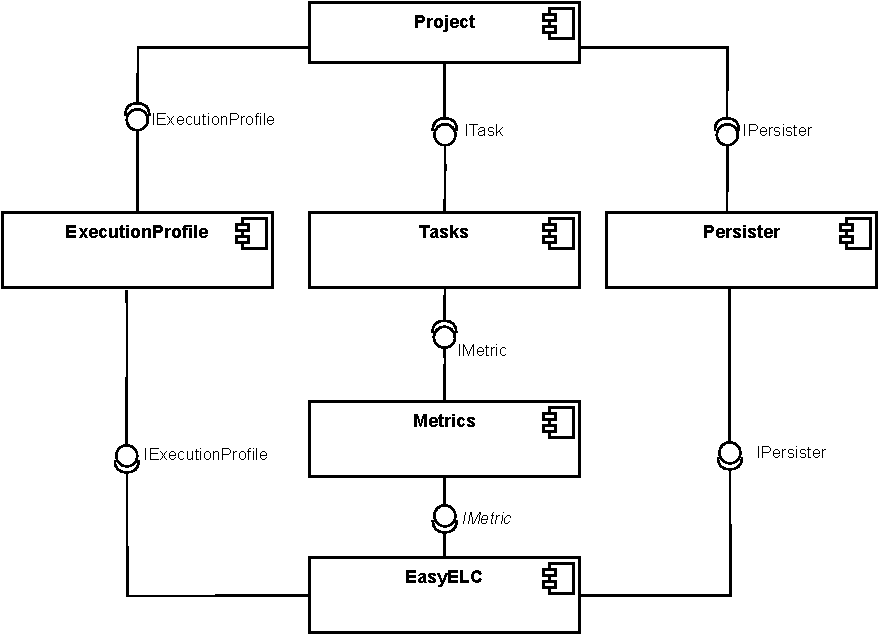
\includegraphics[width=0.6\textwidth]{figures/diagramaarquiteturaelchupacabra.pdf}
	\caption{Diagrama representando os relacionamentos entre os módulos internos da aplicação.}
	\label{fig:diagrama-arquitetura}
\end{figure}

\subsection{Módulo de Projeto (Project)}

O módulo de projeto é o módulo principal da ferramenta, onde o fluxo da coleta é iniciado. Ele é composto somente pela classe Project. Abaixo segue a implementação da classe:

{{IMPLEMENTAÇÃO DA CLASSE PROJECT}}

Essa classe possui como atributos uma instância da classe ExecutionProfile, que contem as informações de quem está executando aquele projeto, uma instância da classe Persister, que é a classe responsável pela persistência de dados, e uma instância da classe Task, que é a tarefa mãe a ser executada.

Possui também um único método, o método executeTask(), que coleta as informações da máquina através do ExecutionProfile, dá inicio a execução das tarefas associadas aquele projeto e persiste os resultados.

\subsection{Módulo de Perfil de Execução (ExecutionProfile)}

A função principal desse módulo é permitir que o usuário consiga coletar informações a respeito do ambiente no qual estão sendo executadas as tarefas. Dessa forma, é possível não só diferenciar os voluntários após a coleta, mas também analisar os ambientes nos quais as tarefas foram executadas. Esse módulo consiste basicamente de uma interface, a IExecutionProfile, e de suas implementações concretas, que representam os tipos de ambientes nos quais as tarefas podem ser executadas. 

{{INSERIR EXEMPLO DE IMPLEMENTAÇÃO DA INTERFACE}}.

Essa interface contém os métodos collect(), que é o método que efetivamente coleta as informações do ambiente, e o método getVisitorId(), que provê um identificador único ao voluntário na execução para posterior análise. Ambos podem ser sobrescritos na implementação concreta de cada perfil, de acordo com a necessidade de cada ambiente.

Supondo uma execução de tarefas em um navegador, deve implementada uma classe chamada BrowserExecutionProfile, que conteria as implementações concretas dos métodos para realizar a coleta dos dados do ambiente do navegador.

{{INSERIR EXEMPLO DE IMPLEMENTAÇÃO DA CLASSE DO BROWSER}}.

\subsection{Módulo de Tarefas (Tasks)}

Esse módulo permite ao usuário implementar tarefas customizadas, sejam elas tarefas simples ou compostas (utilizando o padrão Composite), e também permite a realização de processamentos pré e pós tarefa. Essas tarefas posteriormente são executadas pelo módulo principal de Project.
Assim como o anterior, consiste de uma interface genérica (nesse caso a ITask) e suas implementações concretas. 

{{INSERIR EXEMPLO DE IMPLEMENTAÇÃO DA INTERFACE}}.

A interface ITask contém três métodos principais, que permitem ao usuário criar sua tarefa customizada. O primeiro é o método principal run(), no qual é inserido a chamada para a execução dos jobs e das métricas. Após isso, também são declarados os métodos preTaskJob e postTaskJob, os quais respectivamente representam as execuções que devem rodar antes e depois da tarefa.

A tarefa aqui pode ser desde a transferência de um arquivo, até a execução de uma consulta em um banco de dados. Respeitando a interface principal, podem ser inseritos n tipos de tarefas diferentes, de acordo com a necessidade do usuário. Cada tarefa contém um conjunto de métricas, que são as representações dos tipos de dados que serão coletados na execução daquela tarefa.

Quando houver a demanda de uma tarefa composta por mais de uma tarefa, a implementação se dá utilizando o padrão Composite (citar fundamentação teórica), e a tarefa passa a conter uma lista de tarefas associadas. Assim, quando o método run() é chamado na tarefa mãe, é feita uma iteração nas tarefas associadas para a execução em cadeia de todas as tarefas. 

{{EXEMPLO DE IMPLEMENTAÇÃO DE TAREFA COMPOSTA}}

\subsection{Módulo de Métricas (Metrics)}

O módulo de métricas (Metrics) tem como objetivo representar as métricas que serão coletadas pela ferramenta. Essas métricas estão contidas nas tarefas (Tasks), e são elas as responsáveis de efetivamente coletar o dado desejado do ambiente no qual está sendo executada a tarefa. Esse módulo, assim como os anteriores, consiste de uma interface genérica (nesse caso a interface IMetric) e de suas implementações concretas. Abaixo segue o código base da interface IMetric: 

{{CODIGO DA INTERFACE IMETRIC}}.

A interface principal contém somente um método chamado collect(), que é responsável por executar a coleta efetiva do dado desejado. Extendendo essa interface, a implementação concreta sobrescreve esse método inserindo nele os processamentos necessários para a coleta. Esse método é chamado posteriormente para cada uma das métricas associadas na execução de uma tarefa. Abaixo segue um exemplo de implementação de métrica.

{{EXEMPLO DE IMPLEMENTAÇÃO DE MÉTRICA}}


\subsection{Módulo de Persistência (Persister)}

O módulo de persistência (Persister) tem como finalidade encapsular a persistência de dados após a coleta das métricas, afim de faciltar o uso de diferentes formas de persistência de dados no contexto do framework. Dessa forma, é possível adaptar facilmente a implementação da persistência sem interferir na estrutura das tarefas. Esse módulo é composto pela interface genérica IPersister e suas implementações concretas, assim como os anteriores. Abaixo segue a implementação da interface IPersister.

{{CÓDIGO DA INTERFACE IPERSISTER}}

A interface é composta somente por um método chamado save(), no qual é realizada a persistêcia dos dados propriamente dita. Desse modo, ao instanciar um novo Persister, é nesse método que são realizados os processamentos necessários para salvar o dado da forma desejada. A seguir segue um exemplo de implementação da classe utilizada no exemplo proposto na seção X, o SheetsonPersister.

{{EXEMPLO DE IMPLEMENTAÇÃO DE PERSISTER}}

\subsection{Módulo Simplificado (EasyELC)}


\chapter{Avaliação}
\label{cap:avaliação}

Neste capítulo estão descritos os dois experimentos implementados a fim de testar o projeto em diferentes cenários, cada um deles em sua respectiva secção. A primeira secção, referente ao projeto X, descreve um cenário de implementação mais completo do ELC, e a segunda, referente ao projeto Y, descreve uma abordagem de utilização mais simplificada com o módulo EasyELC, apresentado no capítulo anterior (referenciar a secção da proposta). 

Estudo de caso da tese do Renato


\section{Experimentos}
Experimento envolvendo terceiros? Download de um arquivo... para construir uma visualização




\chapter{Resultados}
\label{cap:resultados}

Nessa secção serão discutidos os resultados dos exemplos propostos para o teste do framework.

\section{Resultado no projeto dos números primos}

Projeto dos números primos.Projeto no qual utilizamos o el-chupacabra de forma mais completa, inclusive usando o Composite nas tasks.


\section{Resultado no site dos números primos utilizando o EasyELC}

Exemplo mais simples, customizando o menos possível, e com um uso mais simplificado. Utilizar a estrutura do EasyELC aplicada no site dos números primos.


\chapter{Conclusão}
\label{cap:conclusão}

Inserir texto

\label{bibpage}
\renewcommand\bibname{Referências}
\addcontentsline{toc}{section}{Referências}
\bibliography{references}
%\bibliographystyle{plainnat}
\bibliographystyle{apalike}
\label{bibfinalpage}

\label{lastpage}



\appendix
\chapter{Prova de Conceito}
\label{apx:mock}

\section{Prova de conceito}
\label{cap:prova_de_conceito}

A fim de testar a modelagem proposta, desenvolvemos uma prova de conceito com objetos mock, os quais simulam recursos computacionais.
De modo que fosse possível avaliar a eficácia da modelagem sem depender de recursos reais, visando manter o foco em avaliar a estrutura do framework.
A prova de conceito foi implementada usando a linguagem de programação Typescript, sua escolha almeja expressar com clareza todas as classes e relações definidas durante a modelagem, e seu código-fonte pode ser encontrado no apêndice \ref{apx:mock_source}.


\subsection{Simulação de Recursos Computacionais}
Como mencionado anteriormente, a prova de conceito possui classes para simular recursos computacionais.
As quais possuem a finalidade de isolar a prova de conceito de complexidades inerentes a realização de medições reais.
Logo, o desenvolvimento da prova de conceito pode ser concentrado em explorar o ponto central da modelagem, a árvore de \emph{Tarefas}.
O bloco de código \ref{lst:mock_memoria} contém a classe criada para simular o consumo de memória.

\begin{lstlisting}[label={lst:mock_memoria}, caption={Implementação da classe responsável por simular recursos de memória para a prova de conceito do framework.}, language=TypeScript]
class Resource {
	private static _total: number = 500;

	static alloc(size: number): any {
		this._total -= size;
		return {size};
	}

	static free(block: any): void {
		this._total += block.size;
	}

	static get total(): number {
		return this._total;
	}
}
\end{lstlisting}


\subsection{Árvore de Tarefas}

A árvore de tarefas é definida basicamente por três classes:
a classe abstrata \emph{Task}, responsável por definir o que uma tarefa faz, ou seja, a sua interface pública.
A classe \emph{CompositeTask}, a qual possui a função de agregar outras tarefas.
E, a classe \emph{SimpleTask}, responsável por encapsular e executar o código do usuário do framework.
Entretanto, tanto \emph{CompositeTask} quanto \emph{SimpleTask} servem apenas para fins de herança e polimorfismo.
Portanto, com o framework em sua completude, as derradeiras classes as quais compõem a árvore de tarefas, serão subclasses.

\begin{lstlisting}[label={lst:abstract_task}, caption={Classe abstrata responsável por definir o que todos os membros da árvore de tarefas precisam implementar.}, language=TypeScript]
abstract class Task {
	public name: string;
	public metrics: Set<Metric<any>>;

	constructor(name: string, metrics: Metric<any>[])
	{
		this.metrics = new Set(metrics);
		this.name = name;
	}

	async run(): Promise<any> {
		this.preTaskJob();
		let data = await this.execute();
		let metrics = {};
		this.metrics.forEach(element => {
		metrics[element.name] = element.metric;
		});
		this.postTaskJob();
		return {metrics, data};
	}

	preTaskJob(): void {};
	abstract execute(): Promise<any>;
	postTaskJob(): void {};
}
\end{lstlisting}

\begin{lstlisting}[label={lst:composite_task}, caption={Tarefa composta, define o comportamento de todos os nós não folha da árvore de tarefas.}, language=TypeScript]
export class CompositeTask extends Task {
	private tasks: Task[];

	constructor() {
		super("Composite Task", []);
		this.tasks = [];
	}

	addTask(task: Task): void {
		this.tasks.push(task);
		task.metrics.forEach(element => {
			this.metrics.add(element);
		});
	}

	async execute(): Promise<any> {
		console.log("Executing composite task...");
		let tasks = {};
		for (const task of this.tasks) {
			tasks[task.name] = await task.run();
		}
		return tasks;
	}
}
\end{lstlisting}


\subsection{Executando a Prova de Conceito}
\label{sec:exe_poc}
A fim de executar a prova de conceito, é necessário criar um arquivo o qual atua como roteiro principal, guiando a execução de outras partes do código.
Além disso, neste mesmo arquivo, é onde construímos a árvore de tarefas.
Ou seja, instanciamos tanto as tarefas compostas quanto às tarefas simples e estabelecemos a sua estrutura de árvore.
Por fim, também é instanciado um objeto \emph{Project} o qual recebe como parâmetros a raiz da árvore de tarefas e uma implementação da interface de persistência.

\begin{lstlisting}[label={lst:index_ts}, caption={Exemplo de roteiro principal para executar a prova de conceito.}, language=TypeScript]
class Index {
	public static async main() {
		console.log("Hello world!");
		const task = new CompositeTask();
		const task2 = new CompositeTask();
		task.addTask(new MockTask("Task 1"));
		task.addTask(new MockTask("Task 2"));
		task2.addTask(new MockTask("Task 3"));
		task.addTask(task2);
		const project = new Project(
			new BasicPersister(),
			task);
		project.executeTask();
	}
}
\end{lstlisting}


\appendix
\chapter{Código-fonte da Prova de Conceito}
\label{apx:mock_source}

\section{Projeto}
\lstinputlisting[language=TypeScript]{./mock/Project.ts}

\section{Index}
\lstinputlisting[language=TypeScript]{./mock/Index.ts}

\section{Tarefa Abstrata}
\lstinputlisting[language=TypeScript]{./mock/Tasks/Task.ts}

\section{Tarefa Composta}
\lstinputlisting[language=TypeScript]{./mock/Tasks/CompositeTask.ts}

\section{Tarefa Simples}
\lstinputlisting[language=TypeScript]{./mock/Tasks/SimpleTask.ts}

\section{Exemplo de implementação de tarefa}
\lstinputlisting[language=TypeScript]{./mock/Tasks/MockTask.ts}

\section{Interface de persistencia}
\lstinputlisting[language=TypeScript]{./mock/Persister/IPersister.ts}

\section{Exemplo de persistencia}
\lstinputlisting[language=TypeScript]{./mock/Persister/BasicPersister.ts}

\section{Mock de tempo}
\lstinputlisting[language=TypeScript]{./mock/Helpers/MockTime.ts}

\section{Mock de Memoria}
\lstinputlisting[language=TypeScript]{./mock/Helpers/MockResource.ts}

\section{Metrica abstrata}
\lstinputlisting[language=TypeScript]{./mock/Metrics/Metric.ts}

\section{Metrica de tempo}
\lstinputlisting[language=TypeScript]{./mock/Metrics/GetDeltaTime.ts}

\section{Metrica de memoria}
\lstinputlisting[language=TypeScript]{./mock/Metrics/GetResourceUsage.ts}

\end{document}